\documentclass[12pt,a4paper]{article}
\usepackage{amsmath,amsfonts,amssymb}
\usepackage{enumerate}
\usepackage{graphicx}
\usepackage{float}
\usepackage{tikz}
\tikzstyle{every node}=[circle, draw, fill=black!50,
	                        inner sep=0pt, minimum width=4pt]

\title{{\bf Graph Theory:}\\
Tutorial 1}
\author{Yaseen Hamdulay \\
	Dean Rance \\
	Sean Wentzel}
\begin{document}
\maketitle
\section*{1.2d}
The order of $Q_t$ is the number of vertices of equal to $2^t$.
The size of $Q_t$ is the number edges. Each vertex has $t$ edges, so the size is $t \times \left(2^{t-1}\right)$ by The First Theorem.

\section*{1.7}
We claim that the result holds.

{\bf Lemma:} If $k<2r$, then there exists a $k$-regular graph on the vertices
$0,1,\dots,2r-1$.

{\bf Proof of Lemma:} If $k$ is even, then let there be an edge from $a$ to $b$
iff $a-b$, taken modulo $2r$, is a member of $S_k=\{-k/2,-k/2+1,\dots,-1,1,\dots,k/2\}$. 
Moreover, since $k/2<r$, none of the members of $S_k$ coincide. In particular,
$|S_k|=k$, and the graph is $k$ regular. Moreover, since $(a+r)-a\equiv_{2r}r \notin S_k$,
the vertices $a$ and $a+r$ (mod $2r$) are not adjacent.

If $k$ is odd, then $k=k_0+1$, with $k_0$ even. Then there exists a $k_0$-regular graph
on $0,1,\dots,2r-1$, described above. To this graph, add edges between $a$ and $a+r$ for
$a=0,1,\dots,r-1$. This increases the degree of each vertex by one, so the resulting graph
is $k$-regular. This concludes the proof of the lemma.

{\bf Main Proof:} Let $T_k$ be a $k$-regular graph on $M=0,1,\dots,2r-1$. We define
$H$ as follows:

$V(H)=M\times V(G)$

$(a,b)(c,d)$ is an edge in $H$ iff either
\begin{itemize}
\item $a=c$ and $bd$ is an edge in $G$
\item $b=d$ and $ac$ is an edge in $T_{r-\text{deg}_G b}$
\end{itemize}
We claim that $H$ is $r$-regular. Consider a vertex $(a,b)$. It can only be adjacent
to a vertex $(c,d)$ in two cases. If $a=c$, then $(a,b)$ is adjacent to $(c,d)$ iff
$bd$ is an edge in $G$. There are $\text{deg}_G b$ such edges. If $b=d$, then $(a,b)$
is adjacent to $(c,d)$ iff $ac$ is an edge in $T_{r-\text{deg}_G b}$, which is
$r-\text{deg}_G b$ regular, so there are $r-\text{deg}_G b$ such edges.
Since $a=c$ and $b=d$ implies $(a,c)=(b,d)$, $(a,c)(b,d)$ is not an edge.
So $\text{deg}_H (a,b) = \text{deg}_G b + r-\text{deg}_G b = r$. Hence $H$ is
$r$-regular.

Finally, let us identify the vertices $(0,b)$ with $b\in V(G)$. We claim that $G$
is induced on these vertices. But $(0,b)(0,d)\in E(H)$ iff $bd \in E(G)$, so this
is clearly true.

Therefore the result holds.


\section*{1.9}
\begin{enumerate}[(a)]
	\item This is not a degree sequence of a graph, as there would be an odd
		number of vertices with odd degrees.
	\item Suppose this was the degree sequence of a graph. Then, by Havel-Hakimi
		theorem, so is $3,2,1,0,0,0$, and $1,0,0,0,0,-1$. But the last is clearly
		not a degree sequence, so the initial sequence is not either.
	\item This is the degree sequence of the graph \\
		\begin{tikzpicture}
			\draw
			(0:1) node {} -- (60:2) node {} -- (0:3) node {}
			(180:1) node {} -- (120:2) node {} -- (180:3) node {}
			(120:2) -- (60:2)
			(240:2) node {} -- (300:2) node {}
			;
		\end{tikzpicture}
	\item Iterations of Havel-Hakimi algorithm go as follows:
\subparagraph{0} 7,4,3,3,2,2,2,1,1,1
\subparagraph{1}   3,2,2,1,1,1,0,1,1
\subparagraph{2}     1,1,0,1,1,0,1,1 which is, of course (with rearrangement), the degree sequence of the graph of $3K_2$ with 2 isolated vertices added.
A graph with the original degree sequence is then \\
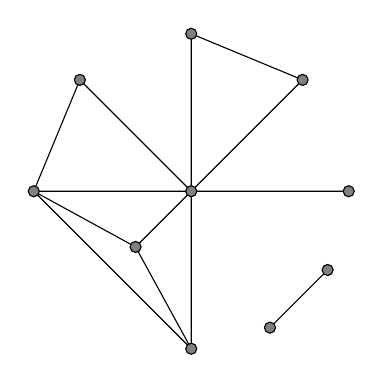
\begin{tikzpicture}
	\draw
	(0:2) node {} -- (0:0) node {} -- (45:2) node {} -- (90:2) node {} -- (0:0)
	(0:0) -- (135:2) node {} -- (180:2) node {} -- (270:2) node {} -- (0:0)
	(0:0) -- (225:1) node {} -- (180:2) -- (0:0)
	(225:1) -- (270:2)
	(300:2) node {} -- (330:2) node {}
	;
\end{tikzpicture}
\end{enumerate}

\section*{1.12}
\begin{enumerate}[(a)]
\item The straight line has only one symmetry on it.
Consider $P_n$, and label its vertices $1,2,\dots, n$, with edge $i,i+1$
for $1 \le i < n$. Now note $1$ and $n$ are the only degree $1$ vertices, so
if $f$ is an automorphism then $f(1)$ is $1$ or $n$. Also, distance
is preserved through automorphism, and that each vertex is uniquely defined by
its distance to $1$, so fixing $f(1)$ fixes the entire automorphism. So there
are at most two automorphisms, the identity and the automorphism taking $i$ to
$n+1-i$. Both of these are clearly automorphisms. When $n=1$, they are not
distinct and there is $1$ automorphism on $P_n$. When $n>1$ they are distinct,
and there are two automorphisms.
\item The cycle $C_n$ has as its automorphism group the dihedral group 
$D_n$, as pointed out in class. $\text{Total} = 2n$
\item Label the vertices $1$ to $n$. Let $\pi_i$ be the permutation
that switches $1$ and $i$ and fixes everything else. Then, since every pair of
vertices is connected, this permutation is an automorphism. Since this is true
for all $i$, the $\pi_i$ generate $S_n$ and the automorphism group is a subgroup
of $S_n$, then the automorphism group is $S_n$
and $\text{Total}=n!$
\item As above, we can generate the automorphism group $S_n$ from 
$2$-cycles. $\text{Total} = n!$
\end{enumerate}

\section*{1.15}
\begin{enumerate}[(a)]
    \item G 
    \begin{figure}[H]
    \centering
    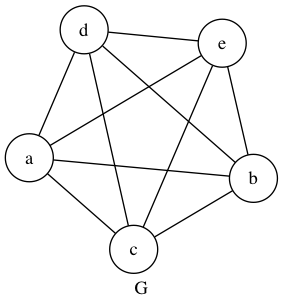
\includegraphics[scale=0.5]{115/115aG.png}
    \end{figure}
    H
    \begin{figure}[H]
    \centering
    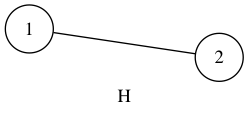
\includegraphics[scale=0.5]{115/115aH.png}
    \end{figure}
    $G+H$
    \begin{figure}[H]
    \centering
    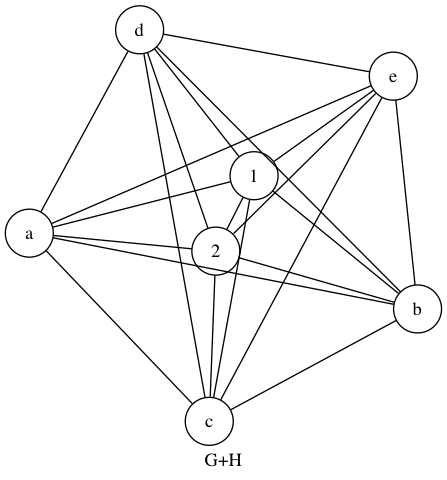
\includegraphics[scale=0.5]{115/115aGH.png}
    \end{figure}
    $GxH$
    \begin{figure}[H]
    \centering
    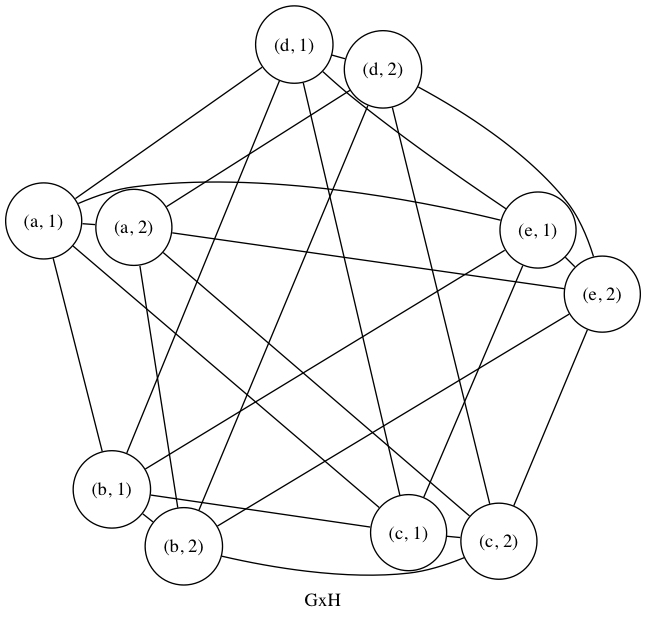
\includegraphics[scale=0.5]{115/115aGH2.png}
    \end{figure}


    \item G 
    \begin{figure}[H]
    \centering
    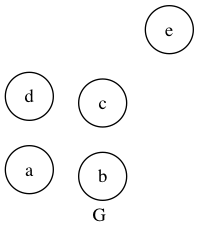
\includegraphics[scale=0.5]{115/115bG.png}
    \end{figure}
    H
    \begin{figure}[H]
    \centering
    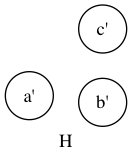
\includegraphics[scale=0.5]{115/115bH.png}
    \end{figure}
    $G+H$
    \begin{figure}[H]
    \centering
    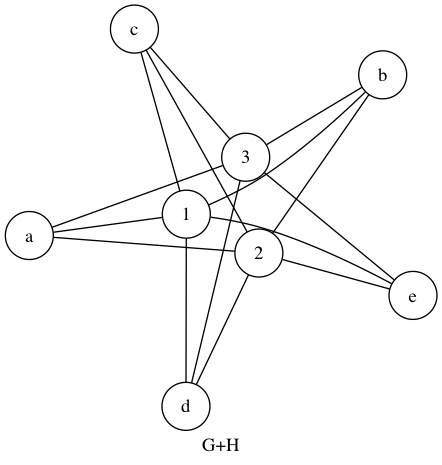
\includegraphics[scale=0.5]{115/115bGH.png}
    \end{figure}
    $GxH$
    \begin{figure}[H]
    \centering
    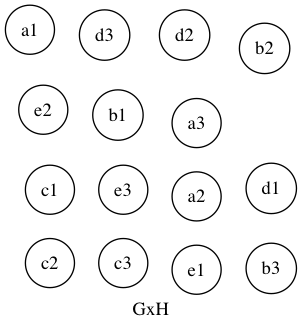
\includegraphics[scale=0.5]{115/115bGH2.png}
    \end{figure}

    \item G 
    \begin{figure}[H]
    \centering
    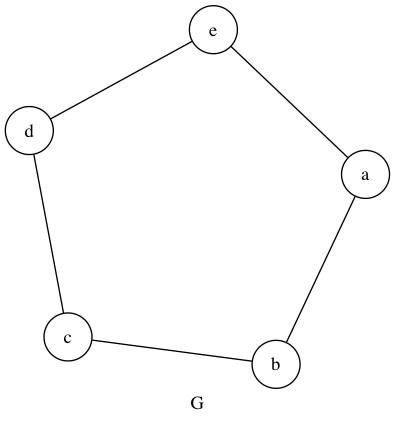
\includegraphics[scale=0.5]{115/115cG.png}
    \end{figure}
    H
    \begin{figure}[H]
    \centering
    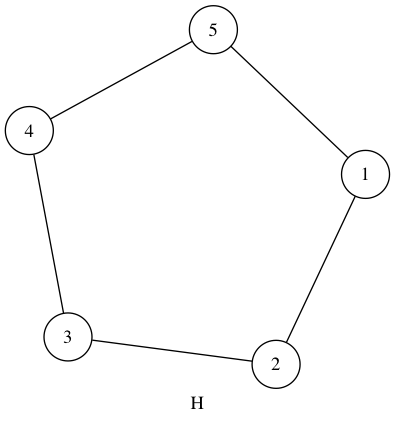
\includegraphics[scale=0.5]{115/115cH.png}
    \end{figure}
    $G+H$
    \begin{figure}[H]
    \centering
    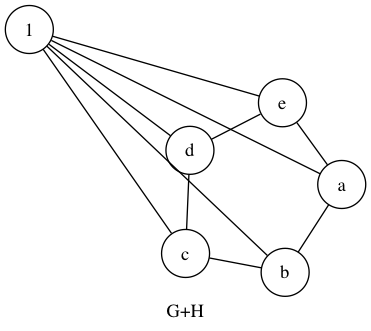
\includegraphics[scale=0.5]{115/115cGH.png}
    \end{figure}
    $GxH$
    \begin{figure}[H]
    \centering
    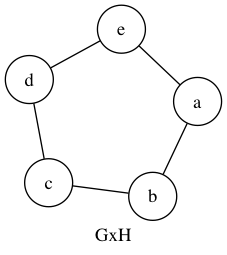
\includegraphics[scale=0.5]{115/115cGH2.png}
    \end{figure}
\end{enumerate}

\section*{1.17}
Choose a vertex $v \in V\left(G\right)$. 
\begin{equation}
d_G\left(v\right) = r 
\end{equation} 
and \begin{equation}
d_{\bar{G}}\left(v\right) = r. 
 \end{equation}
Therefore $|V\left(G\right)| = 2r + 1$, where the 1 is from the vertex we chose.

\section*{1.18}
\paragraph{a}
\subparagraph{order 1}
The trivial graph of order 1 and size 0 is self-complementary.
\subparagraph{order 2}
A graph of order 2 cannot be self-complementary.
\subparagraph{order 3}
Assume that a graph of order 3 is self-complementary. Then, if it has a vertex of degree 0, its complement must have a vertex of degree 0 as well (for this vertex to be mapped to). But that means the original graph has a vertex of degree 2 (whose degree in the complementary graph has degree 0) and so the graph is connected and there is no vertex of degree 0. A graph of order 3 has to have a vertex of either degree 0 or degree 2.
\subparagraph{order 4}
Assume a graph of degree 4 has is self-complementary. If it has a vertex of degree 0, then, as above, it cannot be self-complementary. Thus it also cannot have a vertex of degree 3. So it can only have vertices of degrees 2 and 1. For each vertex with degree 2, its degree in the complementary graph is 1. So for each vertex of degree 2 we need a vertex of degree 1 in the graph. So the only graph to consider is $P_4$. And it is self-complementary.
\subparagraph{order 5}
A graph of order 5 can be self-complementary, if each vertex has degree 2 (i.e. the cycle $C_5$). There is also another graph of degree 5.

\section*{1.19}
\tikzstyle{every node}=[circle, draw, fill=black!50,
	                        inner sep=0pt, minimum width=4pt]
\begin{enumerate}[(a)]
\item \ \\
	
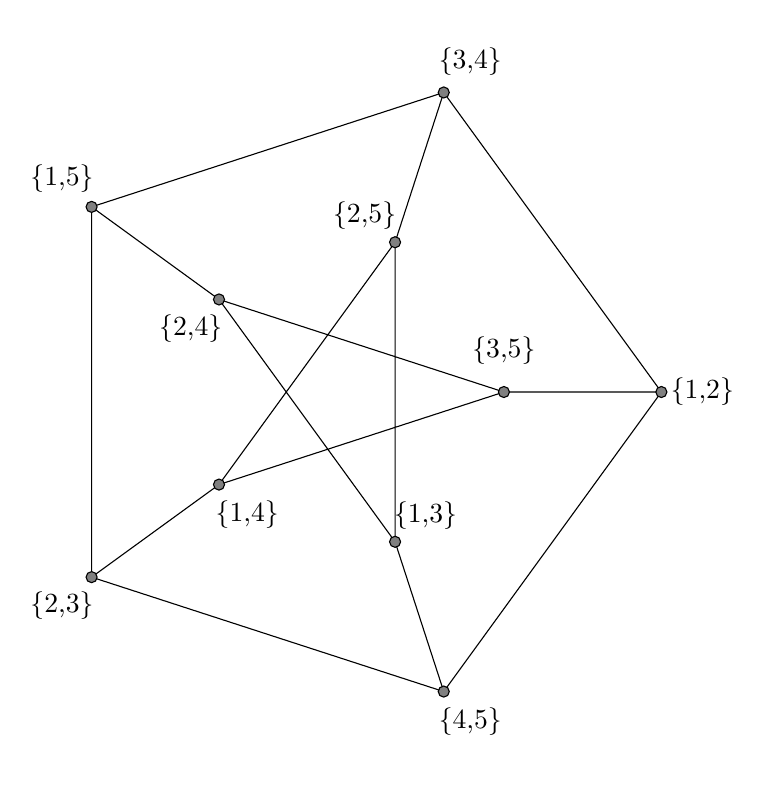
\begin{tikzpicture}
\draw 
(0:2) node [label = {90:\{3,5\}}]{}
(72:2) node [label = {162:\{2,5\}}]{}
(144:2) node [label = {234:\{2,4\}}]{}
(216:2) node [label = {306:\{1,4\}}]{}
(288:2) node [label = {18:\{1,3\}}]{}
(0:4) node [label = {0:\{1,2\}}]{}
(72:4) node [label = {72:\{3,4\}}]{}
(144:4) node [label = {144:\{1,5\}}]{}
(216:4) node [label = {216:\{2,3\}}]{}
(288:4) node [label = {288:\{4,5\}}]{}
\foreach \x in {0,1,...,4} 
{
	(72*\x:2) -- (72*\x:4)
	(72*\x:4) -- (72*\x+72:4)
	(72*\x:2) -- (72*\x+144:2)
};
\end{tikzpicture}

\item The order of $J(n,k,r)$ is just the number of $k$ element subsets of $n$
	elements, or ${n \choose k}$.

\item Let $A$ be a $k$ element subset of $S$. In order to prove that 
	$J(n,k,r)$ is regular, we need show that the number of neighbours of $A$ in
	$J(n,k,r)$ is independent of $A$. But a neighbour of $r$ consists of $r$ vertices
	from $A$ and $k-r$ vertices from $S-A$. We can choose the $r$ vertices of $A$ in
	${k \choose r}$ ways and the $k-r$ vertices of $S-A$ in ${{n-k} \choose {k-r}}$ ways.
	This means the degree of $A$ is ${k \choose r}{{n-k} \choose {k-r}}$, and $J(n,k,r)$
	is regular. By the first
	theorem of graph theory, the size of $J(n,k,r)$ is then just 
	\begin{eqnarray*}
		\frac{1}{2}{n \choose k}{k \choose r}{{n-k} \choose {k-r}} &=& 
		\frac{n!k!(n-k)!}{2k!(n-k)!r!(k-r)!^2(n-2k+r)!}\\
		&=& \frac{n!}{2r!(n-2k+r)!(k-r)!^2}
	\end{eqnarray*}
	if the appropriate binomial coefficients are nonzero. If they are zero (ie when
	$n-k<k-r$) then the graph is completely disconnected.

\item The Petersen graph can be constructed 
	as the complement of the line graph of $K_5$ \cite{petersenwiki}.
	But if the two-element sets making up the vertices of $J(5,2,0)$ are considered
	as edges in $K_5$, then it can be seen that two of them are connected iff they
	are not incident with the same vertex, that is to say
	that $J(5,2,0)$ is precisely the complement
	of the line graph of $K_5$ and hence isomorphic to the Petersen graph.
\end{enumerate}

\end{document}
